
\chapter{Grundlagen}
\thispagestyle{fancy}

\section{Bandstruktur von Gruppe-III Nitriden}

Die wichtige Gruppe der III-Nitridhalbleiter setzt sich aus den Metallen
der dritten Hauptgruppe Aluminium (Al), Gallium (Ga) und Indium (In) zusammen.
Der Schwerpunkt dieser Arbeit liegt auf dem AlGaN-Materialsystem mit hohen Al-Konzentration.
Das Mischverhältnis bestimmt hierbei die Bandlückenergie des Verbindungshalbleiters. Durch die unterschiedlichen Bandlückenergien von Aluminium mit 6.03 eV~\cite{fenaln} und GaN mit 3.4 eV~\cite{pipr} eignet sich AlGaN besonders für die Emission im Wellenlängenbereich von UV-A bis UV-C. 
Die Bandlücke von Verbindungshalbleitern lässt sich durch Interpolation der Bandlückenenergien in Abhängigkeit des Kompositionsverhältnisses x berechnen,
wobei ein zusätzlicher Bowing-Parameter für die nichtlineare Abweichung hinzugefügt wird. 

\begin{equation}
    E_{Al_{x}Ga{1-x}N} = E_{AlN} \cdot x + E_{GaN} \cdot (1-x) - b_{AlGaN} \cdot x \cdot (1-x) 
\end{equation}


\newpage
\section{Polarisationsfeld und QCSE in III/V Halbleitern}
\begin{figure}[htb]
    \centering
    \begin{minipage}[t]{0.49\linewidth}
        \centering
        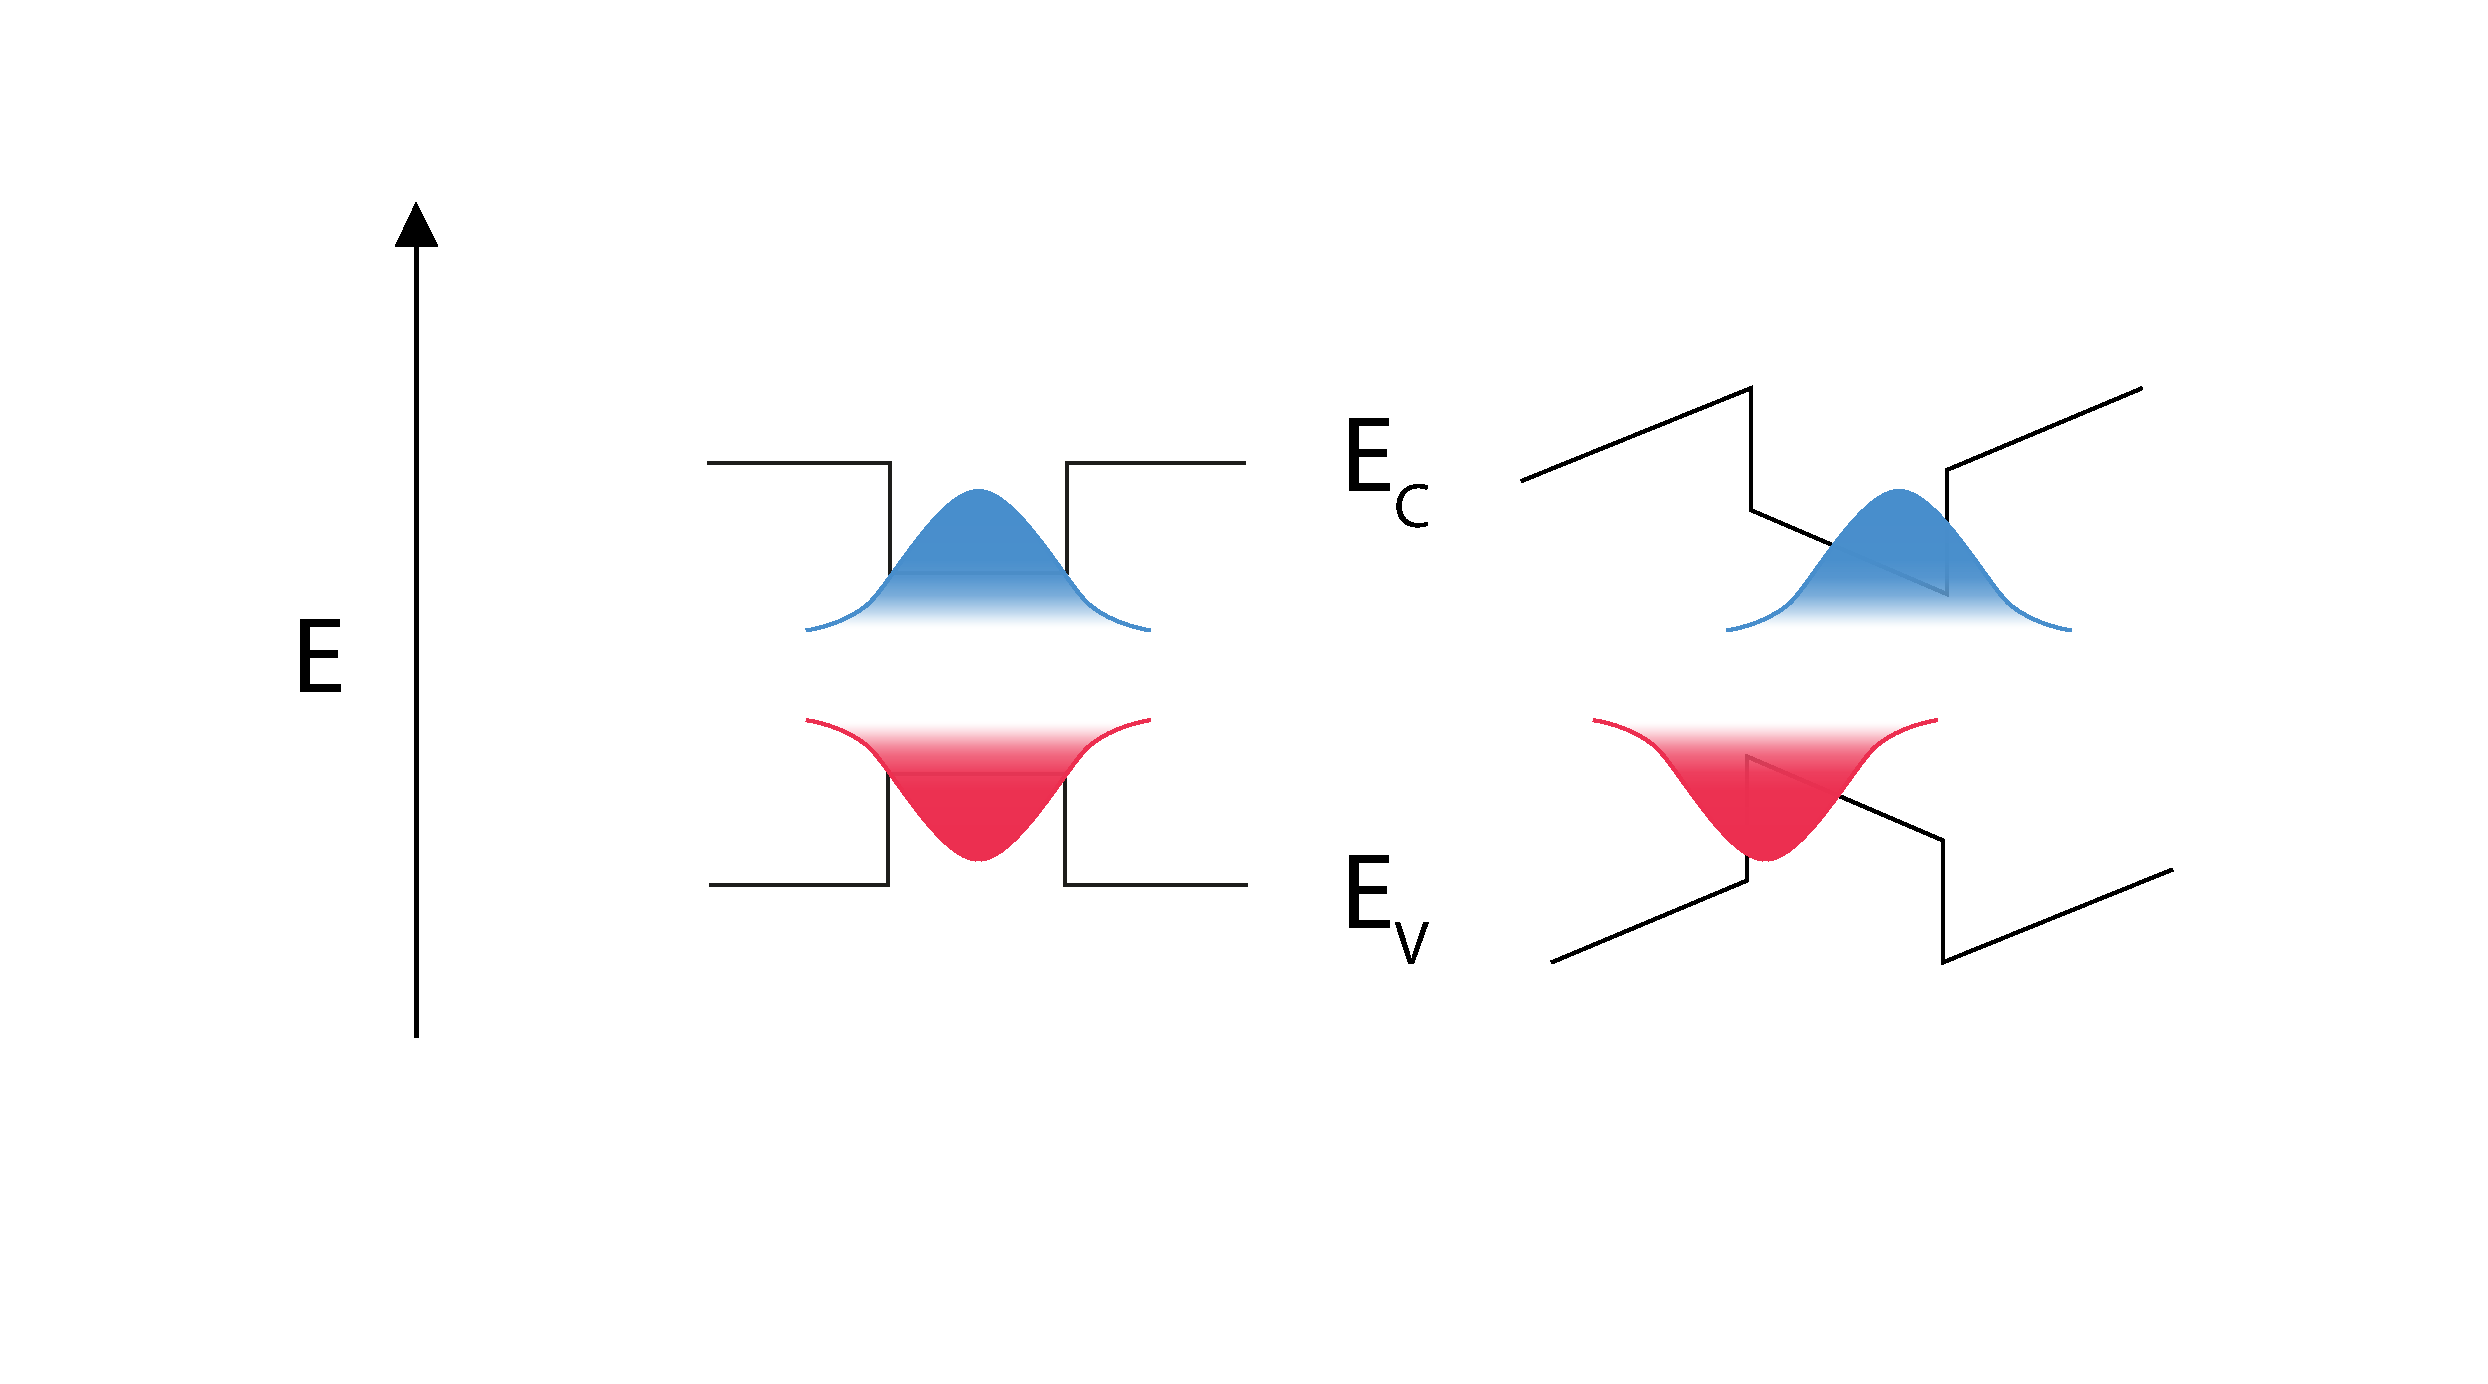
\includegraphics[width=\linewidth]{Bilder/QCSE.pdf}
        \caption{PL-Spektren der Proben ohne Übergitter}
    \end{minipage}% <- sonst wird hier ein Leerzeichen eingefügt
\end{figure}
\vspace{1cm}
\raggedright
Anhand der unterschiedlichen Intensitäten der Proben bei Raumtemperatur sind keine Rückschlüsse zur Effizienz möglich. 
Das liegt zum einen daran, dass die Proben nicht alle auf einen Schlag bei gleichen Bedingungen untersucht wurden und an der Art des Messaufbaus an sich. 
